\documentclass{beamer}
\usepackage{beamerthemesplit}
\usepackage{wrapfig}
\usetheme{SPbGU}
\usepackage{pdfpages}
\usepackage{amsmath}
\usepackage{mathtools}
\usepackage{cmap} 
\usepackage[T2A]{fontenc} 
\usepackage[utf8]{inputenc}
\usepackage[english,russian]{babel}
\usepackage{indentfirst}
\usepackage{amsmath}
\usepackage{tikz}
\usepackage{multirow}
\usepackage[noend]{algpseudocode}
\usepackage{algorithm}
\usepackage{algorithmicx}
\usepackage{ stmaryrd }
\usepackage{qtree}
\usetikzlibrary{shapes,arrows}
\usepackage{fancyvrb}
\usepackage{minted}
\newtheorem{rutheorem}{Теорема}
\newtheorem{ruproof}{Доказательство}
\newtheorem{rudefinition}{Определение}
\newtheorem{rulemma}{Лемма}
\beamertemplatenavigationsymbolsempty

\newcommand{\derive}[0]{\xRightarrow[]{*}}
\newcommand{\derives}[0]{\xRightarrow[]{}}
\newcommand{\derivek}[1]{\xRightarrow[]{#1}}
\newcommand{\deriveg}[1]{\xRightarrow[#1]{*}}
\newcommand{\derivegone}[1]{\xRightarrow[#1]{}}

\title[]{Теория автоматов и формальных языков}
\subtitle[]{Атрибутные грамматики и магазинные преобразователи}
\institute[]{
Санкт-Петербургский государственный электротехнический университет <<ЛЭТИ>>\\
}

\author[]{Екатерина Вербицкая}

\date{29 ноября 2016г.}

\definecolor{orange}{RGB}{179,36,31}

\begin{document}
{
  \begin{frame}
    \titlepage
  \end{frame}
}

\begin{frame}[fragile]
  \transwipe[direction=90]
  \frametitle{В предыдущей серии}
  \begin{itemize}
    \item Полезно не только распознавать предложения или строить деревья их разбора, но и осуществлять трансляцию произвольного вида
    \item Трансляция --- перевод предложения на одном языке в предложение на другом языке
    \item Для этого существует несколько механизмов
    \begin{itemize}
      \item S-атрибутные грамматики
      \begin{itemize}
        \item Все атрибуты синтезируемые (атрибуты узла и его детей)
      \end{itemize}
      \item L-атрибутные грамматики
      \begin{itemize}
        \item Все атрибуты наследуемые (атрибуты узлов предков или братьев слева)
      \end{itemize}
      \item Схема синтаксически управляемой трансляции
    \end{itemize}
    \item Есть ли общий механизм работы с трансляциями?
  \end{itemize}
\end{frame}

\begin{frame}[fragile]
  \transwipe[direction=90]
  \frametitle{В предыдущей серии: простые СУ-схемы}
 Простая схема синтаксически управляемой трансляции --- пятерка $(N, \Sigma, \Pi, P, S)$  
  \begin{itemize}
    \item $N$ --- конечное множество нетерминальных символов
    \item $\Sigma$ --- конечный входной алфавит 
    \item $\Pi$ --- конечный выходной алфавит
    \item $S \in N$ --- стартовый нетерминал
    \item $P$ --- конечное множество правил трансляции вида $A \rightarrow \alpha, \beta$, где $\alpha \in (N \cup \Sigma)^*, \beta \in (N \cup \Pi)^*$
    \begin{itemize}
      \item Нетерминалы входят в цепочку $\beta$ в том же порядке, в каком они входят в $\alpha$
      \item Если нетерминалы повторяются больше одного раза, то их различают по индексам: $E \rightarrow E^l + E^r, + E^l \, E^r$
    \end{itemize}
  \end{itemize}
  
  Такие схемы можно моделировать \textbf{магазинным преобразователем}
\end{frame}

\begin{frame}[fragile]
  \transwipe[direction=90]
  \frametitle{Что такое магазинный преобразователь}
\begin{center}
  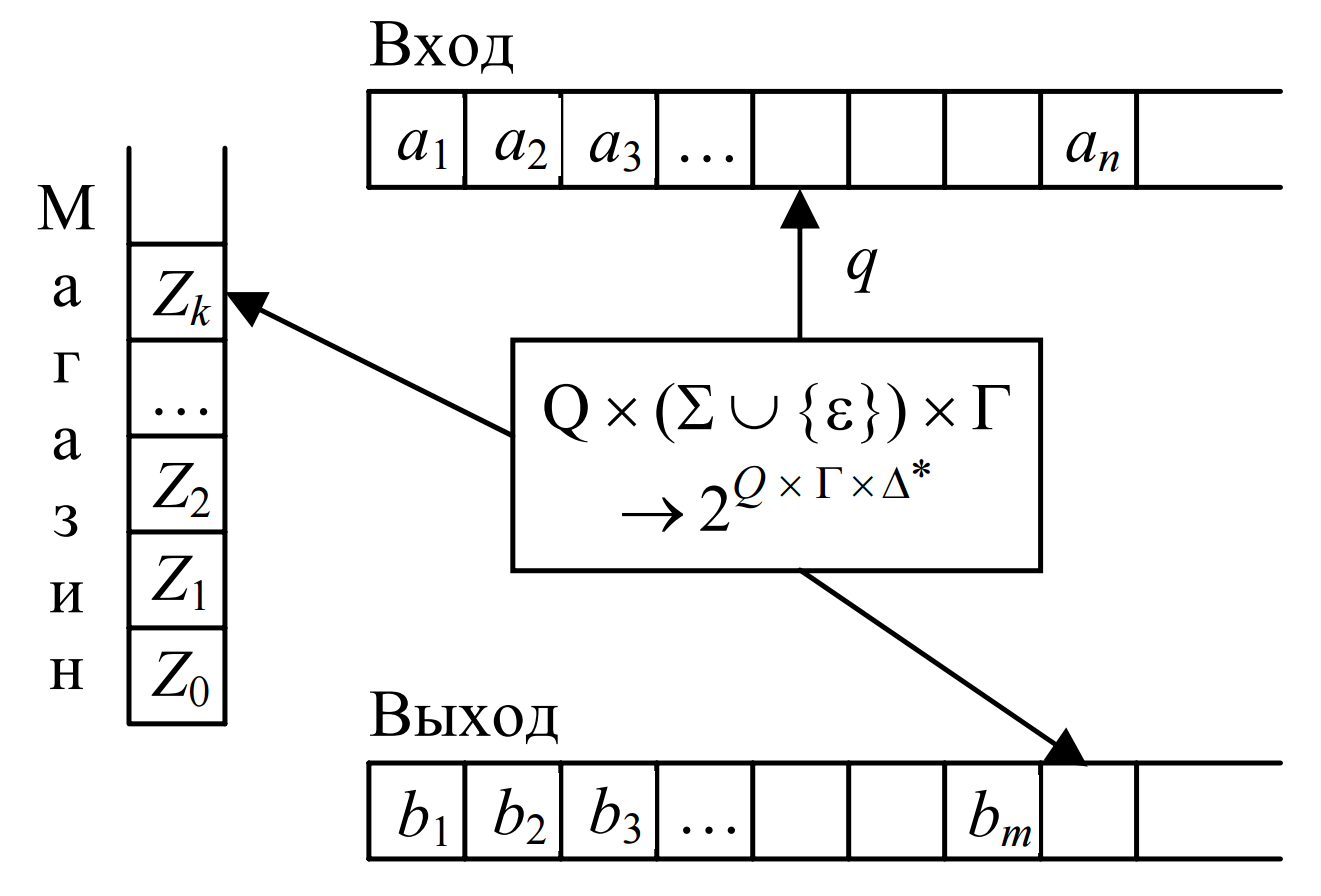
\includegraphics[width=\textwidth]{pics/transducer.png}
\end{center} 

\end{frame}

\begin{frame}[fragile]
  \transwipe[direction=90]
  \frametitle{Что такое магазинный преобразователь: неформально}
\begin{itemize}
	\item Магазинный автомат, который при каждом переходе пишет что-то в выходную строку
\end{itemize}
\end{frame}


\begin{frame}[fragile]
  \transwipe[direction=90]
  \frametitle{Формальное определение}
  Магазинный преобразователь это набор $(Q, \Sigma, \Gamma, \Delta, \delta, q_0, Z_0, F)$
  \begin{itemize}
    \item $Q$ --- конечное множество состояний
    \item $\Sigma$ --- конечное множество символов, входной алфавит
    \item $\Gamma$ --- конечное множество символов, стековый алфавит
    \item $\Delta$ --- конечное множество символов, выходной алфавит
    \item $\delta \subseteq Q \times (Z \cup \varepsilon) \times \Gamma \rightarrow 2^{Q \times \Gamma^* \times \Delta^*}$ --- отношение переходов
    \item $q_0 \in Q$ --- стартовое состояние
    \item $Z_0 \in \Gamma$ --- начальный элемент стека
    \item $F \subseteq Q$ --- множество принимающих (конечных) состояний
  \end{itemize}
\end{frame}

\begin{frame}[fragile]
  \transwipe[direction=90]
  \frametitle{Отношение переходов}
  $\delta(p, a, Z) = \{(q_i, \gamma_i, \alpha_i) \, | \, 1 \leq i \leq n \}$  означает
  \begin{itemize}
    \item Если магазинный преобразователь находится в состоянии $p \in Q$, на вершине стека находится $Z \in \Gamma$, а со входа читается символ $a \in \Sigma \cup \varepsilon$, то для некоторого $i$:
    \begin{itemize}
    	\item Изменяем состояние на $q_i \in Q$
    	\item Снимаем со стека символ $Z$, записываем на стек строку $\gamma_i \in \Gamma^*$
    	\item В выходную строку дописываем $\alpha_i \in \Delta^*$
    \end{itemize}
    \item $\Sigma \cup \varepsilon$ сигнализирует о том, что вход можно и не читать
    \item Если $\gamma_i = \varepsilon$, символ со стека стирается
    \item Если $\alpha_i = \varepsilon$, в выходную строку ничего не пишем
  \end{itemize}
\end{frame}

\begin{frame}[fragile]
  \transwipe[direction=90]
  \frametitle{Семантика магазинного преобразователя}
\begin{itemize}
  \item Мгновенное описание МП: $(p, \omega, \beta, \alpha) \in Q \times \Sigma^* \times \Gamma^* \times \Delta^*$
  \begin{itemize}
  	\item $p$ --- текущее состояние автомата
  	\item $\omega$ --- непрочитанный фрагмент входного потока
  	\item $\beta$ --- содержимое стека (верхушка записана первой)
  	\item $\alpha$ --- содержимое выходной ленты
  \end{itemize}    
  \item Отношение $\vdash$ на мгновенных описаниях (шаг)
  \begin{itemize}
  	\item Для каждого $(q, \gamma, \alpha) \in \delta(p, a, Z)$, верно $(p, a x, Z \eta, \zeta) \vdash (q, x, \gamma \eta, \alpha \zeta)$ для произвольных $x \in \Sigma^*, \eta \in \Gamma^*, \zeta \in \Delta^*$
  \end{itemize}
  \item Шаг не определен, если стек пуст
\end{itemize}

\end{frame}

\begin{frame}[fragile]
  \transwipe[direction=90]
  \frametitle{Семантика магазинного преобразователя: вычисление}
  \begin{itemize}
    \item Вычисление --- последовательность шагов
    \begin{itemize}
      \item $\vdash^*$ --- транизитивно рефлексивное замыкание отношения $\vdash$
    \end{itemize}
    \item Начальное мгновенное описание $(q_0, \omega, Z_0, \varepsilon)$
    \item Два варианта окончания работы
    \begin{itemize}
      \item По достижении конечного состояния
      \begin{itemize}
        \item $\tau(M) = \{ (\omega, \alpha) \, | \, \omega \in  \Sigma^*, \alpha \in \Delta^*, (q_0, \omega, Z_0, \varepsilon) \vdash^* (f, \varepsilon, \gamma, \alpha), f \in F, \gamma \in \Gamma^* \}$
      \end{itemize}
      \item По опустошении стека
      \begin{itemize}
      	\item $\tau_{\varepsilon}(M) = \{ (\omega, \alpha) \, | \, \omega \in  \Sigma^*, \alpha \in \Delta^*, (q_0, \omega, Z_0, \varepsilon) \vdash^* (q, \varepsilon, \varepsilon, \alpha), q \in Q\}$
      \end{itemize}
      \item Эти варианты эквивалентны: по преобразователю, завершающемуся по первой схеме, можно посмотроить преобразователь, завершающийся по второй схеме, и наоборот
    \end{itemize}

  \end{itemize}
\end{frame}

\begin{frame}[fragile]
  \transwipe[direction=90]
  \frametitle{Детерминированные магазинные преобразователи}
  Магазинный преобразователь является \textbf{•}{детерминированным}, если
\begin{itemize}
	\item $\forall q \in Q, a \in \Sigma \cup \{ \varepsilon \}, Z \in \Gamma. | \delta(q, a, Z) | \leq 1$
	\item Если $ \delta(q, \varepsilon, Z) \neq \varnothing$, то $\forall a \in \Sigma. \delta(q, a, Z) = \varnothing$
	\item Детерминированный магазинный преобразователи является частным случаем недетерминированного
\end{itemize}
\end{frame}

\begin{frame}[fragile]
  \transwipe[direction=90]
  \frametitle{Пример: преобразование префиксных арифметических выражений в постфиксные}
$M = \{ \{ q \}, \{ a, +, * \}, \{ E, +, * \}, \{ a, +, * \}, \delta, q, E, \{ q \} \}$



$$
\begin{array}{crcl}
&\delta(q, a, E)& = & \{ (q, \varepsilon, a) \} \\
&\delta(q, +, E)& = & \{ (q, EE+, \varepsilon) \} \\
&\delta(q, *, E)& = & \{ (q, EE*, \varepsilon) \} \\
&\delta(q, \varepsilon, +)& = & \{ (q, \varepsilon, +) \} \\
&\delta(q, \varepsilon, *)& = & \{ (q, \varepsilon, *) \}
\end{array}
$$

$(q, +*aaa, E, \varepsilon) \vdash (q, *aaa, EE+, \varepsilon) \vdash (q, aaa, EE*E+, \varepsilon) \vdash (q, aa, E*E+, a) \vdash (q, a, *E+, aa) \vdash (q, a, E+, aa*) \vdash (q, \varepsilon, +, aa*a) \vdash (q, \varepsilon, \varepsilon, aa*a+)$
\end{frame}

\begin{frame}[fragile]
  \transwipe[direction=90]
  \frametitle{Взаимоотношение между простыми СУ-схемами и магазинными преобразователями}
  \begin{rutheorem}[]
  	По простой СУ-схеме $( N, \Sigma, \Delta, R, S )$  можно построить магазинный преобразователь, задающий эквивалентную трансляцию
  \end{rutheorem}
  
  \begin{rutheorem}[]
    По магазинному преобразователю $P = (Q, \Sigma, \Gamma, \Delta, \delta, q_0, Z_0, \varnothing) $ можно построить простую СУ-схему, задающую эквивалентную трансляцию
  \end{rutheorem}

  \begin{rutheorem}[]
    Класс трансляций, задаваемых простыми СУ-трансляциями совпадает с классом трансляций, задаваемых магазинными автоматами
  \end{rutheorem}
\end{frame}


\begin{frame}[fragile]
  \transwipe[direction=90]
  \frametitle{Однозначные СУ-схемы и левосторонний вывод}
\textbf{Однозначная СУ-схема} --- СУ-схема, в которой не существует двух правил $A \rightarrow \alpha, \beta, A \rightarrow \alpha, \gamma: \beta \neq \gamma$  
  
\begin{rutheorem}[]
Выходная цепочка однозначной СУ-схемы может быть сгенерирована при левостороннем выводе входной цепочки
\end{rutheorem}

\end{frame}

\end{document}
